%latex document

\documentclass[[10pt,abbrv]{llncs}

\usepackage{epsfig}
\usepackage{graphicx}
\usepackage{url}
\usepackage{fancyvrb}
\usepackage{verbatim}
\usepackage{listings}
\usepackage{alltt}
\usepackage{url}
\usepackage{cite}
\DeclareGraphicsExtensions{.png, .jpg, .pdf}
\graphicspath{{./images/}}
\usepackage{array} % Can be used for some tables
\usepackage[table]{xcolor} % For color in tables
\usepackage{makecell} % To make diagonal lines in tables

\usepackage[utf8]{inputenc} % Spanish accent

\begin{document}

\title{A Framework for Multimedia Data-flow Semantic Annotations } %Applications

\author{Natalia~Díaz~Rodríguez, Frank~Wickström, Johan~Lilius}
\institute{Turku Centre for Computer Science (TUCS)\\
Embedded Systems Lab. Department of Information Technologies\\
\AA bo Akademi University, Turku (Finland)\\
{\{ndiaz, frwickst, jlilius}\}@abo.fi}

\maketitle

\begin{abstract}


\end{abstract}

%\keywords
%context-aware, smart space, application development

\section{Introduction}
Modeling complex systems often requires different domain specific languages. Semantic integration makes easier the bridge among synergies.

Defining a language and its generator is considered a difficult task if the aim is building a language for everyone. The task eases considerably if the focus is on one problem domain and domain specific modeling (DSM) can support development and use \cite{Tolvanen2009}. %Some issue to consider is how to motivate this for Smart Spaces if the expert is any kind of domain user?


\section{Domain scenarios to model}

...\\
Another use case of video stream application can be in the bioimaging domain, taking continuous sets of image streams from the microscope for an automatic selection and/or tagging of relevant images. A feedback loop in actions can be modeled with Canals to modify, in real time, the area of interest for which more data is needed.
Some data-flow based use cases in NLP can be the automatic annotation and summarization of text. Given large streams of text, topic disambiguation, summaries and semantics can be obtained for faster processing of information. %Some work in this area can be seen in \cite{}

\section{Description of our data intensive context-aware Use case}


\begin{figure}[tb]
\centering
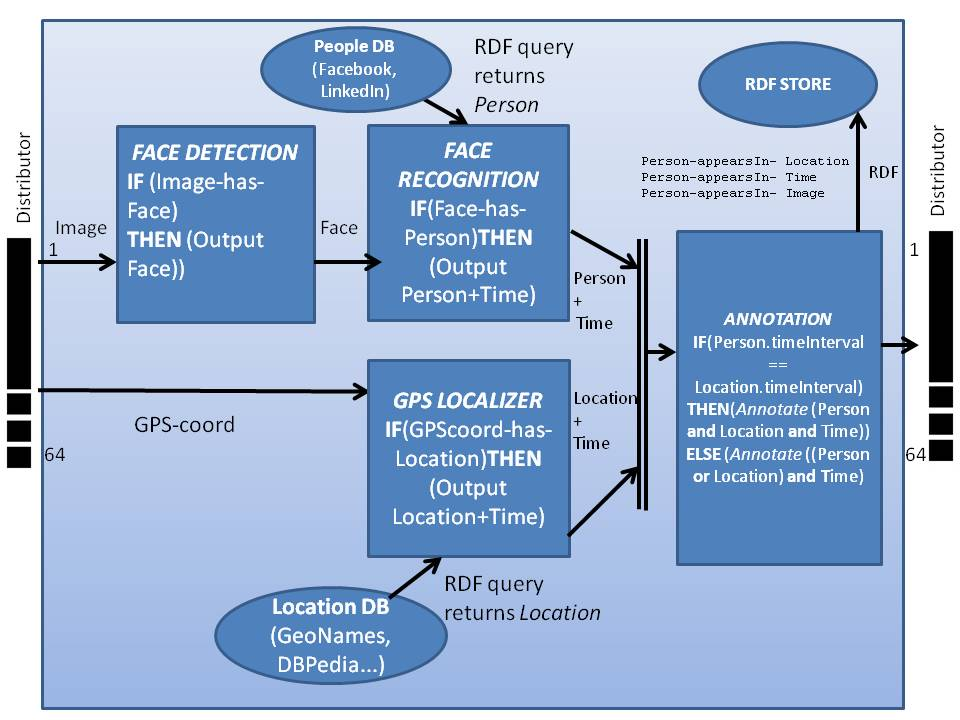
\includegraphics[width=13.5cm]{images/ApplicationEvent-StreamDataflow.jpg}
\caption{Data Stream and Event-based face recognition on a video stream.}
\label{fig:dataflow}
\end{figure}

The diagram in Figure \ref{fig:dataflow} shows how data-stream and event-stream based architectures can be merged to serve such application scenario. The schema uses notation from the Canals language (see next section), and it represents a Canals network which can be mapped to a concrete architecture through its distributors. The network is composed by computation kernels that can be parallelized/scheduled in many-core architectures in order to optimize massive data processing.


\section{Canals, a data-flow language}
Canals \cite{canals} is based on the concept of nodes (kernels and networks) and links (channels), which connect nodes together. Computations are performed in the nodes and the links are representing intermediate buffers in which output data from nodes is stored before the data is consumed by the next node. Canals is implemented in Java and generates code in C. Since Canals is a language independent platform, when a Canals program is mapped to an architecture, the platform independent links are mapped to real connectors on the architecture. Connectors are implemented in the Hardware Abstraction Layer (HAL). HAL consists of stateless low-level functions that triggers underlying hardware mechanisms specific for the underlying platform and the functions used by the dispatchers execute kernels, handle synchronization of kernels/processors and triggers memory transfers. A Canals program without a mapping does not depend on specific hardware synchronization concepts but, instead, only describes the intended behavior of a program in a platform independent manner. Summarizing, the main features of Canals are: the ability to describe scheduling algorithms within the language itself, the implicit deserialization of data at network inputs, and an abstraction layer for synchronization between scheduler and computations.


\section{A multimedia data-flow semantic annotation model}
Our semantic annotation metamodel can be approached in several ways.
\begin{enumerate}
  \item Taking Canals model as a starting point. The description of the Canals language's semantic extension can be done in two ways:
\begin{description}
  \item[a)] Extend Canals metamodel with Java code. Since a metamodel must be done for our semantic annotation architecture, in e.g. EMF, the corresponding generated Java classes can be interfaced with Canals.
  \item[b)] Make Canals metamodel EMF-compatible (since Canals metamodel was designed ad-hoc, manually) and extend Canals EMF metamodel with our semantic annotation metamodel. Since Canals metamodel is much more complex and large in size, manual adaptations of the generated code might easily become a hassle.
\end{description}
 \item Creating an independent semantic annotation metamodel. For this purpose, using UML or OWL modelling languages is a design question. However, a rule engine, production system \footnote{http://en.wikipedia.org/wiki/Production\_system} (i.e. expert system) must be able to become integrated into the system to manage both data-flow and semantic annotation algorithms. Besides, a reasoner will validate the metamodel with, e.g., rules (business rules, etc.).
\end{enumerate}

Taking a bottom-up approach, and focusing on context-aware Smart Space applications, we decide to take approach 2, creating first an independent metamodel in EMF for our semantic framework and providing later an interface with Canals as in option 1.b). This approach leaves flexibility to the semantic annotation metamodel, which could also be run with e.g., another data-flow or parallel language that adapts to certain domain applications, keeping independency in this case of Canals and the semantic annotation framework.
The idea is to start modeling a concrete application model for validation of the semantic metamodel, and then, a schedule could be written in Canals for parallelizing and scheduling a data intensive application.

\begin{figure}[tb]
\centering
\includegraphics[width=12.5cm]{images/annotationUML.png}
\caption{Multimedia Semantic Annotation Metamodel and Model in UML.}
\label{fig:annotationUML}
\end{figure}

In our use case for multiple video tagging, different Interpreters, Concepts and one Environment containing all these is represented in Figure \ref{fig:annotationUML}. Time is an entity that we assumed to be embedded in any GPS input data as well as in any frame header from a video. Therefore, all Interpreters (\verb+FacialDetection, FacialRecognition+ and \verb+GPSLocator+) can perform a Time annotation in parallel to their specific task. Time could be an independent class also though. In cases where Time is not deductible from the direct Observation, an extra Interpreter, e.g., \verb+TimeInterpreter+, could be used for obtaining Time from other available context data.

The metamodel presented in Figure \ref{fig:annotationUML} enables algorithms of different domain to be applied to annotate different kinds of data (image, video, audio, GPS, accelerometer or sensor data, etc.). The execution of the different annotation algorithms is encapsulated in the \verb+Interpreter+ and \verb+Environment+ interfaces, and these could be scheduled and parallelized within Canals; i.e. the methods  \verb+addConcept+ and \verb+addObservation+ will realize all data intensive annotation procedures. The first one adds observations to a certain concept being annotated, and the second, can create further grained Observations from given Observations.
The interface \verb+Environment+ could be one of the only API accessible from Canals code.% (WHAT SHOULD CANALS HAVE ACCESS TO OF THESE CLASSES/INTERFACES?).

\section{System Architecture}
When designing the architecture for a framework with the features described in the previous section, we believe that DSL can ease the task, while ontologies can better formalize the semantics and validity of our model.

\subsection{Domain Specific Languages}
Description Logics based ontology languages are getting more accepted as a means for describing concept structures and constraints, e.g., OWL provides a precise description of the underlying concepts as well as a good bases for reasoning over models in certain domain \cite{Walter2009}. One goal of DSM is to reduce development time. However, since a DSL is much less expressive than e.g. an UML diagram, model elements can be annotated with OWL text and global conditions can be stated using the Manchester OWL Syntax style. After having the whole domain model and its constraints in abstract syntax, the idea, e.g. in \cite{Walter2009}, is to project it to a complete ontology for querying and reasoning.

As metamodeling is a well known way to describe languages \cite{Bezivin01}, and modeling languages such as DSLs must be defined formally to be supported by tools (to be able to generate code from them) \cite{DSM}, our objective is to precisely define the DSLs metamodels and find main connectors for their integration. This allows to define domain models and constraints for model elements simultaneously.


\subsection{Tools for model design and validation}
A model transformation tool \cite{Khan11} that takes as input a UML object model and its class model and produces an ontology, that can be processed by an OWL2 reasoner, can reveal if the object model elements conform to their class model or not.

Two well known metamodeling languages, that target the definition of DSLs, are MOF or UML infrastructures, often used to define the UML or also to define new modeling languages. Other popular metamodeling languages, targeting the definition of DSLs, are Ecore, used in the Eclipse Modeling Framework (EMF) \footnote{http://www.eclipse.org/modeling/emf/}, or KM3. %GEF Plugins for code generation. MOF Script? or in paper OMG-

EMFText OWL2 Manchester Editor, is an Eclipse-based, open-source graphical ontology editor with Pellet integration.

%The EMF (Eclipse Modeling Framework Project) project is a modeling framework and code generation facility for building tools and other applications based on a structured data model. From a model specification described in XMI (XML Metadata Interchange), EMF provides tools and runtime support to produce a set of Java classes for the model, along with a set of adapter classes that enable viewing and command-based editing of the model, and a basic editor.


\subsection{An Ontology for data-flow and context-aware semantic annotations}
Ontologies (represented e.g. by OWL or RDFS languages) have the advantages of supporting other (domain specific) languages by enabling validation or automated consistency checking and having a better support for reasoning than MOF (Meta Object Facility)\footnote{Meta Object Facility, an OMG language for specifying metamodels} based languages \cite{Happel06}.

For the ontology searching task, with the aim of reusing existing work, there are several tools that help us finding present ontologies:
\begin{itemize}
\item OMV: Ontology Metadata Vocabulary \footnote{http://omv.ontoware.org/}.
\item Oyster.
\item Swoogle, Semantic Web Search.
\item Watson.
\item Scarlet - Semantic relations between concepts play an important role in several Semantic Web tasks, such as search, ontology matching, ontology enrichment. Scarlet discovers such relations by exploring the entire Semantic Web as a source of background knowledge. Relying on the functionality of Semantic Web gateways such as Watson or Swoogle, Scarlet automatically finds and combines knowledge provided by multiple online ontologies.
\item Other Ontology Registries.
\end{itemize}

When a candidate  set of ontologies is found, criteria for assessing them needs to be identified.	

In \cite {Hervas10} a formal context model compounded by four independent ontologies (users, devices, environment and services) is presented for describing intelligent environments and enabling interoperability with external ontologies.


Some interesting aspects modeled in \cite{Hervas10} are locations in time, and devices for services and interfaces. This ontology can be reused for the management of embedded resources in the AMEBA project. %See Meta-context 11 and refs of this author, COIVA for visualization.

The state of the art in available context-aware ontologies is well summarized in \cite{Poveda10} as Figure \ref{fig:stateArtContext} shows.
%\begin{figure}[tb]
%\centering
%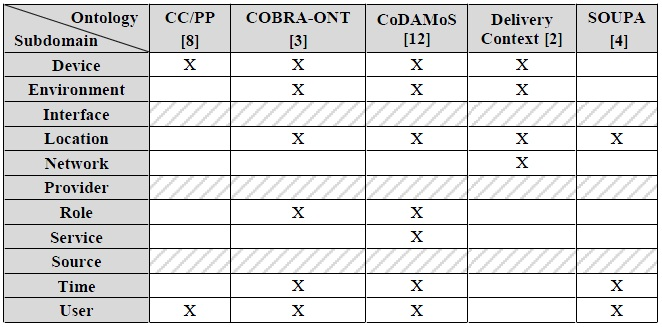
\includegraphics[width=10.5cm]{images/subdomainAddressedByContextOnt.jpg}
%\caption{Subdomain addressed by available context ontologies \cite{Poveda10}.}
%\label{fig:stateArtContext}
%\end{figure}

\begin{table}
\newcolumntype{x}[1]{>{\centering\arraybackslash}p{#1}}
\begin{center}
    \begin{tabular}{|l|x{1.2cm}|x{2.1cm}|x{2cm}|x{1.5cm}|x{1.4cm}|}
    \hline
    \diaghead{\theadfont SubdomainSubdomainnn}%
   {\textbf{Subdomain}}{\textbf{Ontology}}  & \cellcolor[gray]{0.7}CC/PP & \cellcolor[gray]{0.7}Cobra-ONT & \cellcolor[gray]{0.7}CoDAMoS &\cellcolor[gray]{0.7}Delivery Context & \cellcolor[gray]{0.7}SOUPA \\ \hline
    \cellcolor[gray]{0.7}Device & X & X & X & X &  \\ \hline
    \cellcolor[gray]{0.7}Environment & & X & X & X &  \\ \hline
    \cellcolor[gray]{0.7}Interface & \cellcolor[gray]{0.9} & \cellcolor[gray]{0.9} & \cellcolor[gray]{0.9} & \cellcolor[gray]{0.9} & \cellcolor[gray]{0.9} \\ \hline
    \cellcolor[gray]{0.7}Location & & X & X & X & X  \\ \hline
    \cellcolor[gray]{0.7}Network & & & & X &  \\ \hline
    \cellcolor[gray]{0.7}Provider & \cellcolor[gray]{0.9} & \cellcolor[gray]{0.9} & \cellcolor[gray]{0.9} & \cellcolor[gray]{0.9} & \cellcolor[gray]{0.9}  \\ \hline
    \cellcolor[gray]{0.7}Role & & X & X & &  \\ \hline
    \cellcolor[gray]{0.7}Service & & & X & &  \\ \hline
    \cellcolor[gray]{0.7}Source & \cellcolor[gray]{0.9} & \cellcolor[gray]{0.9} & \cellcolor[gray]{0.9} & \cellcolor[gray]{0.9} & \cellcolor[gray]{0.9}  \\ \hline
    \cellcolor[gray]{0.7}Time & & X & X & & X  \\ \hline
    \cellcolor[gray]{0.7}User & X & X & X & & X  \\ \hline
    \end{tabular}  
\end{center}
\label{fig:stateArtContext}
  \caption{Subdomain addressed by available context ontologies \cite{Poveda10}}
\end{table}

We propose an architecture that focuses on observations of certain types, for a context environment to more efficiently process the annotations to be made. Some of the subdomain needed for our domain specific applications are content extraction, online social networks and support for human activity representation.


Next, a context ontology for reasoning with annotated metadata is created. Our focus goes into a location-aware multimedia content. This ontology will allow us having, e.g. a hierarchy of location sources, which will allow reasoning and inferring, for example, of the current position of a person. The provenance of different Location tags could come from FourSquareLocation, WalkbaseLocation,CalendarLocation, GPSLocation, OfficeTrafficLightLocation or FaceLocation (using a FacialRecognition Interpreter and obtaining context from the image).

%Our OWL context ontology proposal can be seen in Figure \ref{fig:contextOWL}:


Some elements modeled on our ontology can be reused from existing ones. These aspect are detailed below.
\begin{itemize}
\item \verb+Time+: the OWL Time ontology, carried out by the Semantic Web Best Practices and Deployment Working Group (SWBPD) from W3C can be reused. However, the extension in \cite{Poveda10} with “Specified Values: Set of Individuals” (LP-SV-01 [15]) pattern allows representing an enumeration of different individuals, e.g., to model the days of the week.
\item \verb+Smart Space+: This class represent an abstraction of a physical space, its semantic repository and its protocols to access it, (including subscription mechanisms). This class can be connected with the general Smart Space model designed for a platform independent Smart Space that contains rules for a rule production system. The general model, based on our previous work \cite{ruSmart}, is sketched in Figure \ref{fig:SSSchema}. This higher hierarchy of the model specifies a general semantic programming platform whose three main interfaces provide flexibility of 1. database (or RDF store), 2. programming language and 3. rule engine. This approach, therefore, does not only ease to program rules in semantic environments, but also through relational databases, noSQL, quads or others. Analogically, it offers to the programmer freedom of choice in reasoning algorithms and rule engines.
\item \verb+Activity+: Human activity recognition based on context-aware ontology reasoning is built on top of our context ontology. Different inferring algorithms can be applied to infer the activity a human is realizing right now.
\item  \verb+User profile preferences+: CC/PP (Composite Capabilities/Preference Profiles) W3C structure and vocabularies. A CC/PP profile is a description of device capabilities and user preferences \footnote{http://www.w3.org/TR/CCPP-struct-vocab/}. On the other side, a W3C Delivery Context Ontology and a glossary of terms for device independence exists but its maintenance was discontinued.
\item  \verb+Online social communities+: The SIOC (Semantically-Interlinked Online Communities) \footnote{http://rdfs.org/sioc/spec} Ontology describes information from online communities (e.g., message boards, wikis, weblogs, etc.) on the Semantic Web. Foursquare check-ins can be managed by using SIOC. It is specially of our interest its view of actions (events) in which a user of an online service acts upon one or several objects of that service.
\item \verb+Content extraction+: Image Annotation W3C \footnote{http://www.w3.org/2005/Incubator/mmsem/XGR-image-annotation/} ontology for semantic image annotation and retrieval can be reused.
\item \verb+Interfaces, devices and services+: The mIO! context ontology is a network ontology that represents the user context to be able to process and use it to configure, discover, execute and enhance different services that the user may be interested in \cite{Poveda10}.
\end{itemize}

There exist specifications for constructing ontology networks \cite{Neon08} when different ontologies can be combined.
Following a methodology to guide ontology development is shown useful \cite{Poveda10}, as well as reusing knowledge resources and attend to good practices in the ontology development. However, reusing context ontologies within a new ontology development becomes difficult due to the different purposes and requirements for which the ontologies are designed.



\begin{figure}[tb]
\centering
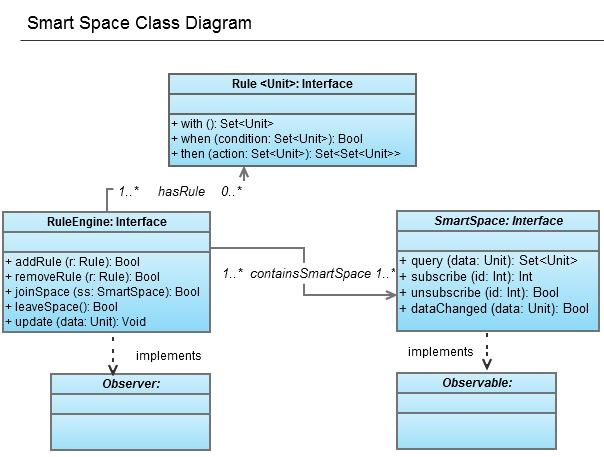
\includegraphics[width=12cm]{images/SmartSpaceIndepArchitecture.jpg}
\caption{General Smart Space Class Diagram.}
\label{fig:SSSchema}
\end{figure}

\section{Related work}

Integration of different DSLs and ontologies using metamodel combination can be seen in \cite{Walter2009}. It shows the merge can be loss-free, containing all information from BDSL (DSL for describing network devices) and FODA (feature description DSL). MetaEdit+ is a tool that integrates modeling and metamodeling approaches for DSLs \cite{Tolvanen2009}.

In \cite{Hoglund10}, metamodels are represented and validated using OWL2 and SWRL. Ordered facts and the closed-world assumptions, available in UML, are represented in OWL2 DL. UML class models and object models are mapped into OWL2 for an automatic validation process with an OWL2 reasoner. %Representing and Validating Metamodels using OWL 2 and SWRL

%There exists a MOF-Based metamodel for OWL2 \footnote{http://www.w3.org/2007/OWL/wiki/MOF-Based\_Metamodel} provided in various formats: owl2.ecore (the metamodel as an Ecore file, can be read e.g. with the open source Eclipse EMF tooling), owl2.emx (the metamodel along with the UML diagrams, can be read e.g. with Rational Software Architect) or owl2.xsd (the XML Schema automatically generated from the metamodel).

The Meta Object Facility (MOF) \footnote{http://www.omg.org/technology/documents/modeling\_spec\_catalog.htm} has proven itself as a valuable and powerful foundation for a family of modeling languages (such as UML, ODM, CWM, etc). However, MOF 2 suffers from the same structural rigidity as many object-oriented programming systems, lacking the ability to classify objects by multiple metaclasses, the inability to dynamically reclassify objects without interrupting the object lifecycle or altering the object's identity and a too constrained view on generalization and properties. MOF Support for Semantic Structures (SMOF) modifies MOF 2 to support dynamically mutable multiple classifications of elements and to declare the circumstances under which such multiple classifications are allowed, required, and prohibited. %This specification is part of the MOF 2 specifications. As such, it does not contain a complete specification of the Meta Object Facility version 2, but an increment to extend the MOF 2 Core with features to handle semantic structures.

%A way of adding semantics to the Canals language metamodel is by integration of the OWL 2 metamodel. OWL 2 Text annotations could be made in Manchester syntax to map concepts and relations among both models as proposed in \cite{Walter2009}.

The TwoUse Toolkit is a toolkit that provides features that support the model driven development and the ontology engineering. OWLizer in TwoUse Toolkit can be used for the generation of an ontology from an annotated Ecore model.
\section{Conclusions and Future work}


\section*{Acknowledgment} The research work presented in this paper is funded by the Academy of Finland through the AMEBA project.

\bibliographystyle{abbrv}
\bibliography{SSReferences}

\end{document} 